

It is based on \textcite{han84} (also mentioned in Sheen (2020) \cite{shee20}).
The nodes are at the same location as for the RT element above, but 
there is an additional bubble function in the middle:

\begin{flushright} {\tiny {\color{gray} (tikz\_han.tex)}} \end{flushright}
%~~~~~~~~~~~~~~~~~~~~~~~~~~~~~~~~~~~~~~~~~~~~~~~~~~~~~~~~~~~~~~~~~~~~~~~~~~~~~~~~~~~~~~~~~~~~~~~~~~



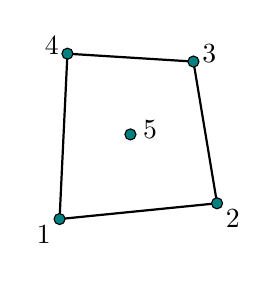
\begin{tikzpicture}
%\draw[fill=gray!23,gray!23](0,0) rectangle (5,5);
%\draw[step=0.5cm,gray,very thin] (0,0) grid (4,4); %background grid
\draw[thick] (1,1) -- (3,1.2) -- (2.7,3) -- (1.1,3.1) -- cycle;  
\node[] at (0.8,0.8) {1};
\node[] at (3.2,1) {2};
\node[] at (2.9,3.1) {3};
\node[] at (0.9,3.2) {4};
\node[] at (2.15,2.13) {5};
\draw[black,fill=teal] (1.9,2.075) circle (2pt);
\draw[black,fill=teal] (1,1)   circle (2pt);
\draw[black,fill=teal] (3,1.2)  circle (2pt);
\draw[black,fill=teal] (2.7,3)  circle (2pt);
\draw[black,fill=teal] (1.1,3.1) circle (2pt);
\end{tikzpicture}




Inside the reference element we assume that a field $f$
can be represented by 
\begin{eqnarray}
f^h(r,s) 
%&=& a+ br +cs +d \phi(r) +e \phi(s) \nn\\
&=& a+ br +cs +d \underbrace{\frac{5r^4-3r^2}{2}}_{\phi(r)}
+e \underbrace{\frac{5s^4-3s^2}{2}}_{\phi(s)} \nn
\end{eqnarray}
We then must have 
\begin{align}
f_1 &= f^h(r=1,s=0) &= a+ b +d \nn\\
f_2 &= f^h(r=0,s=1) &= a+ c +e \nn\\
f_3 &= f^h(r=-1,s=0) &= a- b +d \nn\\
f_4 &= f^h(r=0,s=-1) &= a -c +e \nn\\
f_5 &= f^h(r=0,s=0) &= a  \nn
\end{align}
and we easily get 
\[
a = f_5 
\qquad
f_1-f_3 = 2b
\qquad 
f_2-f_4 = 2c
\]
followed by
\[
d=f_1-a-b = f_1 - f_5 - \frac{1}{2}(f_1-f_3) = \frac{f_1-2f_5+f_3}{2}
\]
and 
\[
e = f_2-a-c = f_2 - f_5 -  \frac{1}{2}(f_2-f_4) = \frac{f_2 -2f_5+f_4 }{2}
\]
Finally:
\[
f(r,s) = 
f_5 +
\frac{1}{2}(f_1-f_3) r+
\frac{1}{2}(f_2-f_4) s+
\frac{f_1-2f_5+f_3}{2} \phi(r)+
\frac{f_2 -2f_5+f_4 }{2} \phi(s)
\]
i.e.
\[
f(r,s) = 
\left(\frac{r + \phi(r)}{2} \right)f_1 +
\left(\frac{s+\phi(s)}{2} \right)f_2 +
\left(-\frac{r-\phi(r)}{2} \right)f_3 +
\left(-\frac{s - \phi(s)}{2} \right)f_4 +
\left(1-\phi(r)-\phi(s) \right)f_5 
\]
which has us define 
\begin{eqnarray}
\bN_1(r,s) &=& \frac{r + \phi(r)}{2} \nn\\
\bN_2(r,s) &=& \frac{s+\phi(s)}{2} \nn\\
\bN_3(r,s) &=& -\frac{r-\phi(r)}{2} \nn\\
\bN_4(r,s) &=& -\frac{s - \phi(s)}{2}\nn\\
\bN_5(r,s) &=& 1-\phi(r)-\phi(s)\nn
\end{eqnarray}
We have of course the following properties $\sum\limits_{i=1}^5 \bN_i(r,s) = 1$ and 
$\bN_i(r_j,s_j) = \delta_{ij},\;  i,j \in 1,5$. 
The partial derivatives of the basis functions are as follows
\begin{eqnarray}
\partial_r \bN_1(r,s) &=& \frac{1 + \phi'(r)}{2} \nn\\
\partial_r \bN_2(r,s) &=& 0 \nn\\
\partial_r \bN_3(r,s) &=& -\frac{1-\phi'(r)}{2} \nn\\
\partial_r \bN_4(r,s) &=& 0 \nn\\
\partial_r \bN_5(r,s) &=& -\phi'(r) \nn\\
\partial_s \bN_1(r,s) &=& 0 \nn\\
\partial_s \bN_2(r,s) &=& \frac{1 + \phi'(s)}{2} \nn\\
\partial_s \bN_3(r,s) &=&  0 \nn\\
\partial_s \bN_4(r,s) &=& -\frac{1-\phi'(s)}{2} \nn\\
\partial_s \bN_5(r,s) &=& -\phi'(s) \nn
\end{eqnarray}
This element is implemented in the {\tt stone\_han.py} file in \stone~77 and also in \stone~120. 






